\chapter{Enhanced Sampling\label{chapter:ES}}
\begin{chapquote}{Bernard R. Brooks%, \textit{\url{https://en.wikiquote.org/wiki/Albert_Einstein}}
	}
	``Keep the smart guys around you.''
\end{chapquote}
From the definition, the free energy of a specific system is dominated by phase space regions with a low potential energy (metastable states). However, these regions might be separated by high energy barriers ($\gg k_BT$). Transitions among these potential energy wells are often hindered by these barriers. According to the Boltzmann's Law, the probability of a sample $\mathbf{R}$ being visited is proportional to the Boltzmann's factor $\exp{\left[-\beta E(\mathbf{R})\right]}$, where $\beta=1/k_BT$ is called the inverse temperature. $k_B$ is the Boltzmann constant and $T$ is the temperature. According to some experience, in a $100\, ns$ simulation, the system can overcome a barrier of $10\, k_BT$, which is $6\, kcal/mol$ at room temperature ($300\, K$). If the barrier is $1.5\, kcal/mol$ higher, it takes about $1\, \mu s$ (10 times longer) in average for the system to go over the barrier. If the barrier height reaches $9\, kcal/mol$, it takes $10\,\mu s$. And so on. As a good practice, convergence should be measured after each simulation.\cite{GrossfieldLJCMS2018}

With modern computers, the longest all-atom molecular dynamics simulation for biological systems is probably the one done by D.E. Shaw, which was on a time scale of 1 ms on a special-purpose computer ``Anton''. For most classical molecular dynamics simulations, the time scales are normally several $\mu s$ to tens of $\mu s$. For simulations using expensive Hamiltonians, such as in QM/MM simulations, the time scales that can be reached are usually three orders shorter. Clearly, molecular dynamics simulations are plagued by a timescale problem. In order to observe abundant transitions among these energy minima, which is required by free energy calculations, enhanced samplings are often indispensable. As shown in the Boltzmann's factor, the essential quantity that determines the rate of transitions is $\beta E$. In order to accelerate the phase space sampling, we can either increase the temperature or decrease the energy barrier. All the methods shown below can be classified into these two categories. Some recent review papers might help.\cite{ZuckermanARB2011,BernardiBBA2015,KamenikPCCP2022,ChenCOSB2022}
\clearpage 
% !TeX spellcheck = en_US
% !TeX encoding = UTF-8
\section{Replica Exchange Molecular Dynamics\label{Sec:ES:REMD}}
\subsection{Temperature-Replica Exchange Molecular Dynamics\label{Sec:ES:REMD:TREMD}}
Temperature replica exchange molecular dynamics (T-REMD) is one class of parallel tempering methods developed by Hansmann, Okamoto and Sugita\cite{HansmannJCC1993,HansmannCPL1997,SugitaCPL1999} based on many ideas in a category of methods called \textit{generalized-ensemble algorithm}. It is an extension of the well-known simulated annealing method. The basic idea of REMD is schematically summarized in Fig.~\ref{Fig:ES:REMD}. In REMD, the system is replicated into $\mathbf{M}$ \textit{non-interacting} copies (replicas). Each replica is coupled to a bath at temperature $T_m$, $(m=1,\dots,M)$. At a certain time, the system is at state X, which can be denoted as $X=\left(x_1^{[i(1)]},\dots,x_M^{[i(M)]}\right)=\left(x_{m(1)}^{[1]},\dots,x_{m(M)}^{[M]}\right)$. Here, we used $i$ and $m$ to label the replica and the temperature respectively. Because the replicas are non-interacting, the weight-factor for a state $X$ in this generalized ensemble is a direct product of the Boltzmann factors for each replica, i.e.
\begin{equation}
	W_{REM}(X)=\prod\limits_{m=1}^M\exp{\left(-\beta_m H\left(q^{[i(m)]},p^{[i(m)]}\right)\right)}=\prod\limits_{i=1}^M \exp{\left(-\beta_{m(i)}H\left(q^{[i]},p^{[i]}\right)\right)}\textsl{}
\end{equation}

\begin{figure}[htbp]
	\centering
	%	\resizebox{2cm}{!}{
	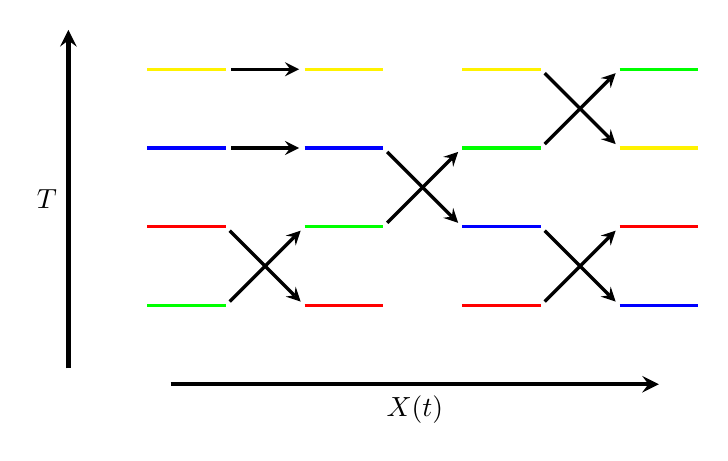
\begin{tikzpicture}
	    \draw[ultra thick,->,>=stealth] (1.3,0) -- (7.5,0) node[midway,below]{$X(t)$};
	    \draw[ultra thick,->,>=stealth] (0,0.2) -- (0,4.5) node[midway,left]{$T$};
	    
        \draw[very thick,green] (1,1) -- (2,1);
        \draw[very thick,red] (1,2) -- (2,2);
        \draw[very thick,blue] (1,3) -- (2,3);
        \draw[very thick,yellow] (1,4) -- (2,4);
        
        \draw[very thick,->,shorten >=2pt,shorten <=2pt,>=stealth] (2,1) -- (3,2);
        \draw[very thick,->,shorten >=2pt,shorten <=2pt,>=stealth] (2,2) -- (3,1);
        \draw[very thick,->,shorten >=2pt,shorten <=2pt,>=stealth] (2,3) -- (3,3);
        \draw[very thick,->,shorten >=2pt,shorten <=2pt,>=stealth] (2,4) -- (3,4);
        
        \draw[very thick,red] (3,1) -- (4,1);
        \draw[very thick,green] (3,2) -- (4,2);
        \draw[very thick,blue] (3,3) -- (4,3);
        \draw[very thick,yellow] (3,4) -- (4,4);
        
        \draw[very thick,->,shorten >=2pt,shorten <=2pt,>=stealth] (4,2) -- (5,3);
        \draw[very thick,->,shorten >=2pt,shorten <=2pt,>=stealth] (4,3) -- (5,2);
        
        \draw[very thick,red] (5,1) -- (6,1);
        \draw[very thick,blue] (5,2) -- (6,2);
        \draw[very thick,green] (5,3) -- (6,3);
        \draw[very thick,yellow] (5,4) -- (6,4);
        
        \draw[very thick,->,shorten >=2pt,shorten <=2pt,>=stealth] (6,1) -- (7,2);
        \draw[very thick,->,shorten >=2pt,shorten <=2pt,>=stealth] (6,2) -- (7,1);
        \draw[very thick,->,shorten >=2pt,shorten <=2pt,>=stealth] (6,3) -- (7,4);
        \draw[very thick,->,shorten >=2pt,shorten <=2pt,>=stealth] (6,4) -- (7,3);
        
        \draw[very thick,blue] (7,1) -- (8,1);
        \draw[very thick,red] (7,2) -- (8,2);
        \draw[very thick,yellow] (7,3) -- (8,3);
        \draw[very thick,green] (7,4) -- (8,4);        
	\end{tikzpicture}
	%	}
	\caption{A schematic representation of replica exchange molecular dynamics.}\label{Fig:ES:REMD}
\end{figure}

%\begin{figure}[htbp]
%    \centering
%	\includegraphics[width=0.6\textwidth]{figures/REMD.pdf}\\
%	\caption{A schematic representation of replica exchange molecular dynamics.}\label{Fig:ES:REMD}
%\end{figure}

Now, we exchange the temperatures of a pair of replicas
\begin{equation}
	\left\{ 
	\begin{array}{rcll} 
		x_m^{[i]}\equiv& \left(q^{[i]},p^{[i]}\right)_m \Rightarrow x_n^{[i]^\prime}&\equiv \left(q^{[i]},p^{[i]^\prime}\right)_n&\\ 
		&&&,\\
		x_n^{[j]}\equiv& \left(q^{[j]},p^{[j]}\right)_n \Rightarrow x_m^{[j]^\prime}&\equiv \left(q^{[j]},p^{[j]^\prime}\right)_m&\\  
	\end{array} 
	\right. 
\end{equation}
where
\begin{equation}
	\left\{ 
	\begin{array}{rl} 
		p^{[i]^\prime}\equiv \sqrt{\frac{T_n}{T_m}} p^{[i]}&\\ 
		&.\\
		p^{[j]^\prime}\equiv \sqrt{\frac{T_m}{T_n}} p^{[j]}&\\  
	\end{array} 
	\right. 
\end{equation}
The exchange rule is not trivial. In order for this exchange process to converge towards an equilibrium distribution, it is sufficient to impose the detailed balance condition on the transition probability $w(X\rightarrow X^\prime)$:
\begin{equation}
	W_{REM}(X)w(X\rightarrow X^\prime) = W_{REM}(X^\prime)w(X^\prime\rightarrow X).
\end{equation}
Then we have
\begin{align}
	&\frac{w\left(X\rightarrow X^\prime\right)}{w\left(X^\prime\rightarrow X\right)}\notag\\
	=&\frac{W_{REM}(X^\prime)}{W_{REM}(X)}\notag\\
	   =&\frac{\exp{\left(-\beta_m H\left(q^{[j]},p^{[j]^\prime}\right)\right)}\exp{\left(-\beta_n H\left(q^{[i]},p^{[i]^\prime}\right)\right)}}{\exp{\left(-\beta_m H\left(q^{[i]},p^{[i]^{ }}\right)\right)}\exp{\left(-\beta_n H\left(q^{[j]},p^{[j]^{ }}\right)\right)}}\notag\\
	   =&\frac{\exp{\left\{-\beta_m\left[K\left(p^{[j]^\prime}\right)+U\left(q^{[j]}\right)\right]-\beta_n\left[K\left(p^{[i]^\prime}\right)+U\left(q^{[i]}\right)\right]\notag\right\}}}
	   {\exp{\left\{-\beta_m\left[K\left(p^{[i]}\right)+U\left(q^{[i]}\right)\right]-\beta_n\left[K\left(p^{[j]}\right)+U\left(q^{[j]}\right)\right]\notag\right\}}}\notag\\
	   =&\frac{\exp{\left\{-\beta_m\left[\frac{T_m}{T_n}K\left(p^{[j]}\right)+U\left(q^{[j]}\right)\right]-\beta_n\left[\frac{T_n}{T_m}K\left(p^{[i]}\right)+U\left(q^{[i]}\right)\right]\notag\right\}}}
	   {\exp{\left\{-\beta_m\left[K\left(p^{[i]}\right)+U\left(q^{[i]}\right)\right]-\beta_n\left[K\left(p^{[j]}\right)+U\left(q^{[j]}\right)\right]\notag\right\}}}\notag\\
	   =&\dfrac{\exp{\left\{-\beta_n K\left(p^{[j]}\right)-\beta_m K\left(p^{[i]}\right)\right\}}}{\exp{\left\{-\beta_m K\left(p^{[i]}\right)-\beta_n K\left(p^{[j]}\right)\right\}}} \dfrac{\exp{\left\{-\beta_m U\left(q^{[j]}\right)-\beta_n U\left(q^{[i]}\right)\right\}}}{\exp{\left\{-\beta_m U\left(q^{[i]}\right)-\beta_n U\left(q^{[j]}\right)\right\}}}\notag\\
	   =&\exp{\left\{-\Delta\right\}}.
\end{align}
where $\Delta = \left[\beta_n-\beta_m\right]\left[U\left(q^{[i]}\right)-U\left(q^{[j]}\right)\right]$. It can be seen that the kinetic energy terms are fully canceled out.
This can be satisfied by the usual Metropolis criterion:
\begin{equation}
	w\left(X\rightarrow X^\prime\right)\equiv w\left(x_m^{[i]}\, \bigg\rvert\, x_n^{[j]}\right)= 
	\left\{ 
	\begin{array}{ll} 
		1, & \text{if } \Delta \leq 0\\ 
		\exp{(-\Delta)}, & \text{if } \Delta >0\\  
	\end{array} 
	\right. 
\end{equation}

The high-temperature replicas and the low-temperature replicas work in a collaborative way, in which the former explore phase space while the latter exploit phase space around local minima. After long time simulations, all the replicas have arrived at a global equilibrium. In order to calculate the free energy or the ensemble average of an operator $\hat A$ at $T_m$, we can extract all the snapshots that have a temperature $T_m$ from $M$ trajectories, if this temperature was among the $M$ chosen temperatures. However, the optimal way is to use Weighted Histogram Analysis Method in Section~\ref{Sec:FEM:WHAM} or the Multistate Bennett Acceptance Ratio method in Section~\ref{Sec:FEM:MBAR}.  

\subsection{Hamiltonian-Replica Exchange Molecular Dynamics\label{Sec:ES:REMD:HREMD}}
Another type of REMD simulation is called Hamiltonian replica exchange molecular dynamics (H-REMD), in which each replicas has its own Hamiltonian, but is coupled to the same temperature.\cite{JangPRL2003} One example is the H-REMD simulation for a torsional angle. The $m$th replica has a torsional energy term of 
\begin{equation}
	H_m(\phi)=\lambda(m)\sum_n\left(V_n/2\right)\left(1+\cos{\left[n\phi-\delta\right]}\right),
\end{equation}
where $\lambda$ is a control parameter. $\lambda(0)=1$ corresponds to the unbiased state and at $\lambda(M)$ (usually $\lambda(M)=0$) the torsional motion of this dihedral angle has a smaller barrier.

Another example of HREMD is pH-REMD, in which each replica is coupled with different pH of the solution. In other words, the chemical potential of hydronium in each replica is different . Therefore, the protonation states (or probability of being protonated or deprotonated) of titratable residues in each replica may differ from those in other replicas. In the simulations, the protonation states of titratable residues have their protonation states alternated according to the Metropolis criterion
\begin{equation}
	P= 
	\left\{ 
	\begin{array}{ll} 
		1, & \text{if } \Delta G_{\ce{P_{A}}\rightarrow \ce{P_{A}H^{+}}}\leq 0\\ 
		\exp{(-\beta\Delta G_{\ce{P_{A}}\rightarrow \ce{P_{A}H^{+}}})}, & \text{if }\Delta G_{\ce{P_{A}}\rightarrow \ce{P_{A}H^{+}}} >0\\  
	\end{array} 
	\right. 
\end{equation}
using Monte Carlo. The derivation of $\Delta G_{\ce{P_{A}}\rightarrow \ce{P_{A}H^{+}}}$ is shown below. 

Free energy of molecule \ce{A} in solution with a concentration $\left[\ce{A}\right]$
can be written as 
\[
\Delta G_{\ce{A}}=\Delta G_{\ce{A}}^{0}+\beta^{-1}\ln\frac{\left[\ce{A}\right]}{C_{0}},
\]
in which $\Delta G_{\ce{A}}^{0}$ is the free energy of molecule A at the standard
state $C_{0}$, i.e. 1 mol/L. The free energy change for a reaction
\begin{center}
	\schemestart \chemfig{A} + \chemfig{B} \arrow{<=>}[,0.75] \chemfig{C} \schemestop
\end{center}
%\[
%A+B\rightleftharpoons C
%\]
can be written as
\[
\Delta G=\Delta G_{\ce{C}}-\Delta G_{\ce{A}}-\Delta G_{\ce{B}}=\Delta G_{0}+\beta^{-1}\ln\frac{\left[\ce{C}\right]C_{0}}{\left[\ce{A}\right]\left[\ce{B}\right]}.
\]

At equilibrium, the free energy change is zero, we have
\begin{equation}
	\Delta G_{0}=-\beta^{-1}\ln\frac{\left[\ce{C}\right]C_{0}}{\left[\ce{A}\right]\left[\ce{B}\right]},\label{eq:FEM:REMD:standardfreeenergy}
\end{equation}
in which $\left[\ce{A}\right]\left[\ce{B}\right]/\left[\ce{C}\right]C_{0}$ is called
the dissociation constant $K_{a}$. So,

\begin{equation}
\Delta G_{0}=\beta^{-1}\ln K_{a}.
\label{eq:FEM:REMD:standardfreeenergyvsKa}
\end{equation}

Titration of a residue in a real protein can be written as
\begin{center}
	\schemestart \chemfig{P_{A}} + \chemfig{H^{+}} \arrow{<=>}[,0.75] \chemfig{P_{A}H^{+}} \schemestop
\end{center}
%\[
%P_{A}+H^{+}\rightleftharpoons P_{A}H^{+},
%\]

with 
\[
K_{a}=\frac{\left[\ce{P_{A}}\right]\left[\ce{H^{+}}\right]}{\left[\ce{P_{A}H^{+}}\right]C_{0}}
\]

The fraction of the deprotonated species is calculated as

\begin{eqnarray}
	f_{\left[\ce{P_{A}}\right]} & = & \frac{\left[\ce{P_{A}}\right]}{\left[\ce{P_{A}}\right]+\left[\ce{P_{A}H^{+}}\right]}\nonumber \\
	& = & \frac{1}{1+\frac{\left[\ce{P_{A}H^{+}}\right]}{\left[\ce{P_{A}}\right]}}\nonumber \\
	& = & \frac{1}{1+\frac{\left[\ce{P_{A}}\right]\left[\ce{H^{+}}\right]}{C_{0}K_{a}\left[\ce{P_{A}}\right]}}\nonumber \\
	& = & \frac{1}{1+\frac{1}{C_{0}K_{a}}\left[\ce{H^{+}}\right]}\nonumber \\
	& = & \frac{1}{1+\frac{1}{K_{a}}10^{-\mathrm{pH}}}\label{eq:FEM:REMD:titrationcurve}
\end{eqnarray}
We can check the asymptotic behavior of this equation. At strong
acidic condition ($\mathrm{pH}=-\infty$), $f_{\left[\ce{P_{A}}\right]}=0$, indicating that
the residue is 100 percent protonated. While at an extremely basic
condition ($\mathrm{pH}=\infty$), $f_{\left[\ce{P_{A}}\right]}=1$. This residue is 100
percent deprotonated. From the Henderson–Hasselbalch (HH) equation, 
the $\mathrm{p}K_a$ can be determined by the $\mathrm{pH}$ of the state when 
$\left[\ce{P_{A}}\right]/\left[\ce{P_{A}H^{+}}\right]=1$

\begin{align}
	\mathrm{p}K_{a}  = & -\log{K_{a}}\notag\\
	 = & -\log{\frac{\left[\ce{P_{A}}\right]}{\left[\ce{P_{A}H^{+}}\right]}}-\log{\frac{\left[\ce{H^{+}}\right]}{C_{0}}}\notag\\
	 = & -\log{\frac{\left[\ce{P_{A}}\right]}{\left[\ce{P_{A}H^{+}}\right]}}+\mathrm{pH}.
	 \label{eq:FEM:REMD:pKa}
\end{align}
The $\mathrm{p}K_{a}$ of each residue in a dipeptide has been determined by
experiment. However, when this residue is located in a certain protein,
its $\mathrm{p}K_{a}$ is different from that in the dipeptide. The difference
is called the $\mathrm{p}K_{a}$ shift. Instead of measuring the $\mathrm{p}K_{a}$
for a residue in a protein, we are more interested in calculating/measuring
the titration curve, which is the fraction of the deprotonated state
as a function of pH. From Eq.~\ref{eq:FEM:REMD:titrationcurve}, $f_{\left[P_{A}\right]}$
can be easily calculated if we know $K_{a}$ or equivalently the standard
free energy change of protonation in Eq.~\ref{eq:FEM:REMD:standardfreeenergyvsKa}.
The standard free energy can be calculated from the partition functions
as

\begin{eqnarray*}
	\Delta G_{0} & = & -\beta^{-1}\ln\frac{Q_{\ce{P_{A}H^{+}}}}{Q_{\ce{P_{A}}}Q_{\ce{H^{+}}}}\\
	& = & -\beta^{-1}\ln\frac{\iint\exp(-\beta E_{\ce{P_{A}H^{+}}})\diff \mathbf{R}_{H}\diff \mathbf{R}_{o}}{Q_{\ce{H^{+}}}\int\exp(-\beta E_{\ce{P_{A}}})\diff \mathbf{R}_{o}},
\end{eqnarray*}
where $\mathbf{R}_{H}$ is the coordinates of the specific \ce{H} atom and the other degrees-of-freedom (DoF) are denoted as $\mathbf{R}_{o}$. Generally, the absolute value of $\Delta G_{0}$ is hardly computable. A relative protonation free energy $\Delta\Delta G$ is preferred and is more reliable. Theoretically, the reference state can be any state you like. But the protonation free energy of the dipeptide is often used. The reference protonation process can be written as
\begin{center}
	\schemestart \chemfig{A} + \chemfig{H^{+}} \arrow{<=>}[,0.75] \chemfig{AH^{+}} \schemestop
\end{center}
%\[
%A+H^{+}\rightleftharpoons AH^{+}.
%\]

The free energy change from the reference state is 

\begin{align}
	&\Delta\Delta G_{0}\nonumber\\
	= & \Delta G_{0}-\Delta G_{0}^{ref}\nonumber \\
	= & -\beta^{-1}\ln\frac{\iint\exp(-\beta E_{\ce{P_{A}H^{+}}})\diff \mathbf{R}_{H}\diff \mathbf{R}_{o}}{Q_{\ce{H^{+}}}\int\exp(-\beta E_{\ce{P_{A}}})\diff \mathbf{R}_{o}}\frac{Q_{\ce{H^{+}}}\int\exp(-\beta E_{\ce{A}})\diff \mathbf{R}_{o}}{\iint\exp(-\beta E_{\ce{AH^{+}}})\diff \mathbf{R}_{H}\diff \mathbf{R}_{o}}\nonumber \\
	= & -\beta^{-1}\ln\frac{\iint\exp(-\beta E_{\ce{P_{A}H^{+}}})\diff \mathbf{R}_{H}\diff \mathbf{R}_{o}\int\exp(-\beta E_{\ce{A}})\diff \mathbf{R}_{o}}{\int\exp(-\beta E_{\ce{P_{A}}})\diff \mathbf{R}_{o}\iint\exp(-\beta E_{\ce{AH^{+}}})\diff \mathbf{R}_{H}\diff \mathbf{R}_{o}}\nonumber \\
	= & -\beta^{-1}\ln\frac{\iint\exp{\left[-\beta \left(E_{\ce{P_{A}H^{+}}}^{bond}+E_{\ce{P_{A}H^{+}}}^{QM}+E_{\ce{P_{A}H^{+}}}^{ele}\right)\right]}\diff \mathbf{R}_{H}\exp\left(-\beta E_{\ce{P_{A}H^{+}}}^{other}\right)\diff \mathbf{R}_{o}}{\iint\exp\left[-\beta \left(\ce{E_{AH^{+}}}^{bond}+E_{\ce{AH^{+}}}^{QM}+E_{\ce{AH^{+}}}^{ele}\right)\right]\diff \mathbf{R}_{H}\exp\left(-\beta E_{\ce{AH^{+}}}^{other}\right)\diff \mathbf{R}_{o}}\nonumber \\
	 & \cdot\frac{\int\exp\left(-\beta E_{\ce{A}}\right)\diff \mathbf{R}_{o}}{\int\exp\left(-\beta E_{\ce{P_{A}}}\right)\diff \mathbf{R}_{o}},\label{eq:FEM:REMD:Quotientofpartitionfunctions}
\end{align}
where $E^{bond}$
and $E^{ele}$ are the bonded energy and electrostatic interaction
energy related to this \ce{H} atom, respectively. $E^{QM}$ is the energy
correction that \textit{may} be required if the molecular mechanical
Hamiltonian cannot well capture the energy of the system, such as
the missing of charge transfer effect. The sum of the remaining energy
term is denoted as $E^{other}$, which does not explicitly depend
on the position of this specific \ce{H} atom. Eq.~\ref{eq:FEM:REMD:Quotientofpartitionfunctions}
is not ready to be computed before some approximations are adopted. 

\textit{First}, we assume that the total energy can be well described by the MM Hamiltonians
for both the state interested in and the reference state. Therefore,
\[
E_{\ce{P_{A}H^{+}}}^{QM}=E_{\ce{AH^{+}}}^{QM}=Const,
\]
and they can be removed from the integral. 

\textit{Second}, the bonded terms involving hydrogen atoms are usually 
constrained in the simulations. Therefore, the hydrogen atom in question has 
only one position and $E^{bond}=0$. Now, the 
relative protonation free energy can be simplified as
\begin{align}
\Delta\Delta G_{0}=&-\beta^{-1}\ln\frac{\int\exp\left(-\beta E_{\ce{P_{A}H^{+}}}^{ele}\right)\exp\left(-\beta E_{\ce{P_{A}H^{+}}}^{other}\right)\diff \mathbf{R}_{o}}{\int\exp\left(-\beta E_{\ce{AH^{+}}}^{ele}\right)\exp\left(-\beta E_{\ce{AH^{+}}}^{other}\right)\diff \mathbf{R}_{o}}\notag\\
&\cdot\frac{\int\exp\left(-\beta E_{\ce{A}}\right)\diff \mathbf{R}_{o}}{\int\exp\left(-\beta E_{P_{\ce{A}}}\right)\diff \mathbf{R}_{o}}.
\end{align}

Note that $E_{\ce{A}}=E_{\ce{AH^{+}}}^{other}$ and $E_{\ce{P_{A}}}=E_{\ce{P_{A}H^{+}}}^{other}$, we have
\begin{align}
	\Delta\Delta G_{0} = & -\beta^{-1}\ln\frac{\int\exp\left(-\beta E_{\ce{P_{A}H^{+}}}^{ele}\right)\exp\left(-\beta E_{\ce{P_{A}}}\right)\diff \mathbf{R}_{o}}{\int\exp\left(-\beta E_{\ce{P_{A}}}\right)\diff \mathbf{R}_{o}}\\
	& \cdot \frac{\int\exp\left(-\beta E_{\ce{A}}\right)\diff \mathbf{R}_{o}}{\int\exp\left(-\beta E_{\ce{AH^{+}}}^{ele}\right)\exp\left(-\beta E_{\ce{A}}\right)\diff \mathbf{R}_{o}}\\
	= & -\beta^{-1}\ln\left\langle \exp\left(-\beta E_{\ce{P_{A}H^{+}}}^{ele}\right)\right\rangle _{\ce{P_{A}}}\notag\\
	  &+\beta^{-1} \ln\left\langle \exp\left(-\beta E_{\ce{AH^{+}}}^{ele}\right)\right\rangle _{\ce{A}}\notag\\
	= & \Delta G_{\ce{P_{A}H^{+}}}^{ele}-\Delta G_{\ce{AH^{+}}}^{ele}  
\end{align}

Therefore,
\[
-\beta^{-1}\ln10\cdot \mathrm{p}K_{a}=\Delta G_{\ce{P_{A}H^{+}}}^{ele}-\Delta G_{\ce{AH^{+}}}^{ele}-\beta^{-1}\ln10\cdot \mathrm{p}K_{a}^{ref}.
\]

Using Eq.~\ref{eq:FEM:REMD:pKa}, at a certain pH the free energy difference between the deprotonated
and the protonated state can be written as

\[
\Delta G_{\ce{P_{A}}\rightarrow \ce{P_{A}H^{+}}}=\Delta G_{\ce{P_{A}H^{+}}}^{ele}+\beta^{-1}(\mathrm{pH}-\mathrm{p}K_{a}^{ref})\ln10-\Delta G_{\ce{AH^{+}}}^{ele}.
\]

In the above equation, $\Delta G_{\ce{AH^{+}}}^{ele}$ can be obtained from a free energy calculation of the model system by alchemically annihilation of the proton. However, $\Delta G_{\ce{P_{A}H^{+}}}^{ele}$ is unknown. Approximately, it can be replaced with $\Delta H_{\ce{P_{A}H^{+}}}^{ele}$ averaged over a few snapshots.\cite{MengJCTC2010} In order to accelerate the convergence,
this pH-REMD is often coupled with other enhanced simulation methods, such as T-REMD\cite{MengJCTC2010} and EDS-REMD\cite{LeeJCTC2014} (see section~\ref{Sec:ES:EDS}).
\clearpage
% !TeX spellcheck = en_US
% !TeX encoding = UTF-8
\section{Simulated Tempering\label{Sec:ES:ST}}
Simulated tempering (ST) was proposed by Marinari and Parisi\cite{MarinariEPL1992} and by Lyubartsev et al\cite{LyubartsevJCP1992} in 1992, and by Geyer and Thompson\cite{GeyerJASA1995} in 1995. In ST, there is only one trajectory with controlled jumps in temperature space, which is different from the implementation of T-REMD\ref{Sec:ES:REMD:TREMD}, in which multiple trajectories are running in parallel. In ST, the simulation is carried out in an extended space defined by the configuration variables $\mathbf{X}$ and a new variable $m$. The latter can take $M$ values ($m=1,\dots,M$). Corresponding to each $m$, there is an inverse temperature $\beta_m$. Let
\begin{equation}
    \beta_0>\beta_1>\beta_2>\cdots >\beta_m.
\end{equation}
The probability distribution $\rho(\mathbf{X},m)$ will be chosen to be 
\begin{equation}
  \rho(\mathbf{X},m)\propto \exp{\left[-H(\mathbf{X},m)\right]}
\end{equation}
with 
\begin{equation}
  H(\mathbf{X},m)\equiv \beta_m H(X)-g_m.
\end{equation}
The total partition function for this extended ensemble is
\begin{align}
    Z=&\sum_{m=1}^M \int\diff \mathbf{X} \exp{\left[-H(\mathbf{X},m)\right]}\notag\\
     =&\sum_{m=1}^M \int\diff \mathbf{X} \exp{\left[-\beta_m H(X)+g_m\right]}\notag\\
     =&\sum_{m=1}^M \exp{(g_m)}\int\diff \mathbf{X} \exp{\left[-\beta_m H(X)\right]}
\end{align}

For each $\beta_m$, there is a canonical ensemble with the probability for a configuration $\mathbf{X}$ follows the usual Boltzmann distribution, i.e. 
\begin{equation}
    \rho(X|m)\propto \exp{(-\beta_m H(X))}.
\end{equation}
and the partition function (with $1/N!$ omitted)
\begin{equation}
    Z_m=\int \diff \mathbf{X} \exp{[-\beta_m H(\mathbf{X})]}=\exp{(-\beta_m f_m)}.
\end{equation}
where $f_m$ is the associated free energy. With this definition of $Z_m$, the total partition function can be written as
\begin{equation}
    Z=\sum_{m=1}^M \exp{(g_m)} Z_m,
\end{equation}
where $\exp{(g_m)}$ can be thought as the weight for the $m$th canonical ensemble in this extended ensemble.

On the other hand, the probability of having a given value of $m$ is simply given by
\begin{equation}
    \rho_m=\frac{\int\diff \mathbf{X} \exp{\left[-H(\mathbf{X},m)\right]}}{Z}=\frac{Z_m\exp{(g_m)}}{Z}=\frac{1}{Z}\exp{(-\beta_m f_m+g_m)}.
\end{equation}
If we make the choice $g_m=\beta_m f_m$, then all the $\rho_m$ become equal. However, $f_m$ is usually unknown beforehand, or it may be never known.

The system may evolve in two types of steps: (1) usual displacements of particles at fixed temperature via molecule dynamics or Monte Carlo and (2) changes of reciprocal temperature with fixed positions of particles. In the first case, detailed balance can be easily maintained. In the second case, in order to maintain detailed balance
\begin{equation}
    \rho(\mathbf{X},m)P(\beta_m\to \beta_{m\pm 1}|\mathbf{X})=\rho(\mathbf{X},m\pm 1)P(\beta_{m\pm 1}\to \beta_{m}|\mathbf{X}),
\end{equation}
transition takes place with the probability
\begin{equation}
    P(\beta_m\to \beta_{m\pm 1}|\mathbf{X})=\min{\left\{1,\exp{\left[-(\beta_{m\pm1}-\beta_m)H(\mathbf{X})+(g_{m\pm1}-g_m)\right]}\right\}}
\end{equation}
following the Metropolis criteria.
\clearpage
% !TeX spellcheck = en_US
% !TeX encoding = UTF-8
\section{Umbrella Sampling\label{Sec:ES:US}}
Umbrella Sampling method was proposed by Torrie and Valleau in 1977,\cite{TorrieJComputP1977} and is still widely used nowadays.
Suppose we are studying a transition process between two states such as conversion between two dominant conformations or a chemical reaction, and these two states are separated by a high barrier relative to $k_BT$. Therefore, the transition is a rare event. A schematic representation of the free energy landscape is shown in Fig.~\ref{Fig:ES:dual_harmonic}.
\begin{figure}[htbp]
	\centering
%	\resizebox{2cm}{!}{
		\begin{tikzpicture}
		\def\lims{xmin=-5,xmax=5,ymin=-30,ymax=14}
		\begin{axis}[\lims,hide x axis, hide y axis,width=0.65\textwidth,height=0.4\textwidth]
           \addplot[mark=none,smooth,domain=-5:5] {0.4*((x+2)*(x-2))*((x+2)*(x-2))-4*x*x};
		\end{axis}
		\end{tikzpicture}
%	}
	\caption{A typical free energy surface. Two free energy wells are separated by a barrier higher than $k_BT$.}\label{Fig:ES:dual_harmonic}
\end{figure}

%\begin{figure}[htbp]
%	\centering
%	\includegraphics[width=0.6\textwidth]{figures/dual_harmonic.pdf}\\
%	\caption{A typical free energy surface. Two free energy barriers are separated by a barrier higher than $kT$.}\label{Fig:ES:dual_harmonic}
%\end{figure}

Sometimes, we are interested in not only these two dominant states but also the whole pathway. Usually, we define a reaction coordinate $\xi$, including one or more collective variables (CVs), which can distinguish the two minima and characterize the free-energy pathway. Then we want to know the free-energy change along the reaction coordinate, $\xi$. It should be noted that choosing a suitable set of CVs is nontrivial for most cases.\cite{LeitoldJCP2020} A CV can be either a real coordinate such as the difference of bond lengths in, for example, an $S_N2$ reaction, or a thermodynamics coupling parameter ($\lambda$) that defines an unphysical path. If we run a simulation with the reaction coordinate set to a local maximum, i.e. the system being the transition state, the system will quickly roll back to the ``reactant'' or the ``product'' state in order to reduce the free energy. The consequence is that phase space outside the ``reactant'' and ``product'' regions cannot be sampled sufficiently to yield accurate free energy profile in a brute force simulation. In order to enhance the exploration in these regions, we can added a bias potential $\Delta V(\xi)$ into the system, guaranteeing
\begin{equation}
	\forall \xi_{1} \; \mathrm{and} \; \xi_{2}, \left [ U(\xi_{1}) + \Delta V(\xi_{1}) \right ]  - \left [ U(\xi_{2}) + \Delta V(\xi_{2}) \right ] < k_BT
\end{equation}
then the free-energy surface can be explored within the timescale amenable to MD simulations. $\Delta V(\xi)$ is called the ``umbrella potential''.

However, as the free-energy surface is usually not known \textit{a priori}, it is difficult to determine $\Delta V(\xi)$. To circumvent this issue, we can stratify the free-energy pathway into multiple \textit{windows}, namely break up the reaction-coordinate space into ``parts'', by a series of (usually harmonic) restraints, $\Delta U_i(\xi)$. In other words, the $i$th simulation, or the simulation of the $i$th window, is performed on the potential energy surface 
\begin{equation}
	U_i(\mathbf{R})=U_0(\mathbf{R})+\Delta U_i(\xi).
\end{equation}
The strengths of the biases should be strong enough to maintain the system in the vicinity of where you are interested in, and also should be weak enough that the system can have significant overlap between two adjacent windows. At the same time, the windows should be small enough to guarantee in each window,
\begin{equation}
	\forall \xi_{1} \; \mathrm{and} \; \xi_{2}, \left [ U(\xi_{1}) + \Delta U_i(\xi_{1}) \right ]  - \left [ U(\xi_{2}) + \Delta U_i(\xi_{2}) \right ] < k_BT
\end{equation}
After all the simulations, the (biased) distribution of the samples in the whole region should be as flat as possible. Ensemble average under $U_0$ can be calculated from the ensembles generated under the biased Hamiltonians $U$ via
\begin{align}
	\left<X(\mathbf{R})\right>_0=&\frac{\int X(\mathbf{R})\exp{\left[-\beta U_0(\mathbf{R})\right]}\diff\mathbf{R}}{\int \exp{\left[-\beta U_0(\mathbf{R})\right]}\diff\mathbf{R}}\notag\\
	                            =&\frac{\int X(\mathbf{R})\exp{\left[\beta \Delta U_i(\mathbf{R})\right]}\exp{\left[-\beta U_i(\mathbf{R})\right]}\diff\mathbf{R}}{\int \exp{\left[\beta \Delta U_i(\mathbf{R})\right]}\exp{\left[-\beta U_i(\mathbf{R})\right]}\diff\mathbf{R}}\notag\\
	                =&\frac{\left<X\exp{\left(\beta\Delta U_i\right)}\right>_i}{\left<\exp{\left(\beta\Delta U_i\right)}\right>_i}.
	\label{Eq:ES:US:reweighting}
\end{align}
Better postprocessing methods are the Weighted Histogram Analysis Method, Umbrella Integration and the Multistate Bennett Acceptance Ratio method (to be discussed in Section~\ref{Sec:FEM:WHAM}, ~\ref{Sec:FEM:UI} and~\ref{Sec:FEM:MBAR}).
\clearpage
% !TeX spellcheck = en_US
% !TeX encoding = UTF-8
\section{Accelerated Molecular Dynamics\label{Sec:ES:aMD}}
Accelerated molecular dynamics, or aMD for short, was proposed by Hamelberg et al in 2004.\cite{HamelbergJCP2004}

In this method, the simulation is performed on the modified potential $V^\ast(\mathbf{r})$
\begin{equation}
	V^\ast(\mathbf{r})= 
	\left\{ 
	\begin{array}{rl} 
		V(\mathbf{r}), &\quad V(\mathbf{r})\geq E\\ 
		V(\mathbf{r})+\Delta V(\mathbf{r}), &\quad V(\mathbf{r})< E\\  
	\end{array} 
	\right.
\end{equation}
in which $E$ is a certain chosen energy, $\Delta V(\mathbf{r})$ is a continuous non-negative boost potential function, and $V(\mathbf{r})$ is the true potential. The bias potential increases the escape rate of the system from potential basins, and the subsequent state to state evolution of the system on the modified potential occurs at an accelerated rate with a nonlinear time scale of $\Delta t^\ast_i$, where
\begin{equation}
	\Delta t^\ast_i=\Delta t_i e^{\beta \Delta V(\mathbf{r}(t_i))}.
\end{equation}
The ensemble average value of any observable $A(\mathbf{r})$ taken on the modified potential can be written as
\begin{align}
	\left<A^\ast\right>=&\frac{\int \diff \mathbf{r}\,A(\mathbf{r})e^{-\beta V^{\ast}(\mathbf{r})}}{\int \diff \mathbf{r}\, e^{-\beta V^{\ast}(\mathbf{r})}}\notag\\
	        =&\frac{\int \diff \mathbf{r}\,A(\mathbf{r})e^{-\beta V(\mathbf{r})-\beta \Delta V(\mathbf{r})}}{\int \diff \mathbf{r}\, e^{-\beta V(\mathbf{r})-\beta \Delta V(\mathbf{r})}}.
\end{align}
The correct ensemble average can be written as
\begin{align}
	\left<A\right>=&\frac{\int \diff \mathbf{r}\,A(\mathbf{r})e^{-\beta V(\mathbf{r})}}{\int \diff \mathbf{r}\, e^{-\beta V(\mathbf{r})}}\notag\\
	=&\frac{\int \diff \mathbf{r}\,A(\mathbf{r})e^{-\beta V^\ast(\mathbf{r})+\beta \Delta V(\mathbf{r})}}{\int \diff \mathbf{r}\, e^{-\beta V^\ast(\mathbf{r})+\beta \Delta V(\mathbf{r})}}\notag\\
	=&\frac{\left<A(\mathbf{r})e^{\beta \Delta V(\mathbf{r})}\right>_{V^\ast}}{\left<e^{\beta \Delta V(\mathbf{r}) }\right>_{V^\ast}}.
\end{align}
Some technique can improve the numerical stability of this reweighting process.\cite{MiaoJCTC2014} The definition of $\Delta V(\mathbf{r})$ is non-unique, and Hamelberg et al proposed a modification of the potential energy surface more akin to snow drifts, which smooths the landscape by filling minima, but maintains the underlying shape of the unmodified potential energy surface and merges smoothly with the original potential at the threshold ``boost energy'' value $E$. It is defined as
\begin{equation}
	\Delta V(\mathbf{r})=\frac{(E-V(\mathbf{r}))^2}{\alpha+(E-V(\mathbf{r}))},
\end{equation}
where $\alpha$ is a tuning parameter that determines how deep the modified potential energy basin is (when $E-V(\mathbf{r})=\alpha, \Delta V(\mathbf{r})=\alpha/2$). With this biasing potential, the derivative of $V^{\ast}(\mathbf{r})$ has no discontinuity, and the modified potential reproduces the shape of the minima even at high value of $E$. Furthermore, $E$ should be carefully chosen, which may require a short trial simulation.

The most recent variant of aMD, the Gaussian accelerated molecular dynamics (GaMD), was developed by Miao et al\cite{MiaoJCTC2015}, in which the biasing potential is defined as
\begin{equation}
	\Delta V(\mathbf{r})= 
	\left\{ 
	\begin{array}{rl} 
		\frac{1}{2}k(E-V(\mathbf{r}))^2, &\quad V(\mathbf{r})< E\\ 
		0, &\quad V(\mathbf{r})\geq E\\  
	\end{array} 
	\right.
\end{equation}

In order to smoothen the potential energy surface for enhanced sampling, the boost potential needs to satisfy the following criteria. First, for any two arbitrary potential values $V(\mathbf{r}_1)$ and $V(\mathbf{r}_2)$ found on the original energy surface, $\Delta V$ should be a monotonic function that does no change the relative order of the biased potential values, i.e. 
\begin{equation}
	\sign{(V(\mathbf{r}_1)-V(\mathbf{r}_2))}=\sign{(V^\ast(\mathbf{r}_1)-V^\ast(\mathbf{r}_2))}.
\end{equation}
Without losing generality, let $V(\mathbf{r}_1)<V(\mathbf{r}_2)$, we have
\begin{equation}
	V^\ast(\mathbf{r}_1)<V^\ast(\mathbf{r}_2),
\end{equation}
which leads to
\begin{align}
    V(\mathbf{r}_1)+\frac{1}{2}k\left[E-V(\mathbf{r}_1)\right]^2-V(\mathbf{r}_2)-\frac{1}{2}k\left[E-V(\mathbf{r}_2)\right]^2<&0\notag\\
    \left[V(\mathbf{r}_1)-V(\mathbf{r}_2)\right]+\frac{1}{2}k\left[(2E-V(\mathbf{r}_1)-V(\mathbf{r}_2))(V(\mathbf{r}_2)-V(\mathbf{r}_1))\right]<&0\notag\\
    \left[V(\mathbf{r}_1)-V(\mathbf{r}_2)\right]\left[1-\frac{1}{2}k(2E-V(\mathbf{r}_1)-V(\mathbf{r}_2))\right]<&0.
\end{align}
Since $V(\mathbf{r}_1)<V(\mathbf{r}_2)$, we have
\begin{equation}
	1-\frac{1}{2}k(2E-V(\mathbf{r}_1)-V(\mathbf{r}_2))>0,
\end{equation}
or equivalently
\begin{equation}
	\text{Criterion 1: } E<\frac{1}{k}+\frac{1}{2}\left[V(\mathbf{r}_1)+V(\mathbf{r}_2)\right].
\end{equation}

Second, if $V(\mathbf{r}_1)<V(\mathbf{r}_2)$, the potential difference observed on the smoothened energy surface should be smaller than that of the original; i.e., $V^\ast(\mathbf{r}_2)-V^\ast(\mathbf{r}_1)<V(\mathbf{r}_2)-V(\mathbf{r}_1)$, which leads to
\begin{equation}
	\text{Criterion 2: } E>\frac{1}{2}\left[V(\mathbf{r}_1)+V(\mathbf{r}_2)\right].
\end{equation}
Therefore, the threshold energy must satisfy
\begin{equation}
	V_{\mathrm{max}}\leq E \leq V_{\mathrm{min}}+\frac{1}{k},
\end{equation}
where $V_{\mathrm{max}}$ and $V_{\mathrm{min}}$ are the maximum and minimum of potential energies, and $k$ has to satisfy
\begin{equation}
	k\leq \frac{1}{V_{\mathrm{max}}-V_{\mathrm{min}}}.
\end{equation}
It can be rewritten as
\begin{equation}
	k=k_0\frac{1}{V_{\mathrm{max}}-V_{\mathrm{min}}},
\end{equation}
where $k_0\in (0,1)$. $k_0$ determines the magnitude of the applied boost potential. With greater $k_0$, higher boost potential is added to the potential energy surface. The boost potential is
\begin{equation}
	\Delta V(\mathbf{r})=\frac{1}{2} k_{0} \frac{1}{V_{\max }-V_{\min }}(E-V(\mathbf{r}))^{2}, \quad V(\mathbf{r})<E.
\end{equation}

Third, the standard deviation of $\Delta V$ needs to be small enough (i.e., narrow distribution) to ensure accurate reweighting using cumulant expansion to the second order:\cite{MiaoJCTC2014}
\begin{equation}
	\sigma_{\Delta V}=\sqrt{\left(\left.\frac{\partial \Delta V}{\partial V}\right|_{V=V_{\mathrm{av}}}\right)^{2} \sigma_{V}^{2}}=k\left(E-V_{\mathrm{av}}\right) \sigma_{V} \leq \sigma_{0},
\end{equation}
where $V_{av}$ and $\sigma_{V}$ are the average and standard deviation of the system potential energies, and $\sigma_{\Delta V}$ is the standard deviation of $\Delta V$ with $\sigma_{0}$ as a user-specified upper limit (e.g., $10k_BT$) for accurate reweighting. If $E$ is set to the lower bound $E=V_{\mathrm{max}}$, we have
\begin{equation}
	k_{0} \leq \frac{\sigma_{0}}{\sigma_{V}} \frac{V_{\max }-V_{\min }}{V_{\max }-V_{\mathrm{av}}}.
\end{equation}
For efficient enhanced sampling with the highest possible acceleration, $k_0$ can then be set to its upper bound as
\begin{equation}
	k_{0}=\min \left(1.0, \frac{\sigma_{0}}{\sigma_{V}} \frac{V_{\max }-V_{\min }}{V_{\max }-V_{\mathrm{av}}}\right).
\end{equation}
Alternatively, when the threshold energy $E$ is set to its upper bound $E = V_{\mathrm{min}} + (1/k)$, we have
\begin{equation}
	k_{0} \geq\left(1-\frac{\sigma_{0}}{\sigma_{V}}\right) \frac{V_{\max }-V_{\min }}{V_{\mathrm{av}}-V_{\min }}.
\end{equation}
Then, we have
\begin{equation}
	\text{Criterion 3: } \left(1-\frac{\sigma_{0}}{\sigma_{V}}\right) \frac{V_{\max }-V_{\min }}{V_{\mathrm{av}}-V_{\min }} \leq k_0 \leq \frac{\sigma_{0}}{\sigma_{V}} \frac{V_{\max }-V_{\min }}{V_{\max }-V_{\mathrm{av}}}.
\end{equation}
\clearpage
% !TeX spellcheck = en_US
% !TeX encoding = UTF-8
\subsection{Adaptive Biasing Force Method\label{Sec:ES:ABF}}
Adaptive biasing force method was proposed by Darve and Pohorille in 2001.\cite{DarveJCP2001}.
\clearpage 
% !TeX spellcheck = en_US
% !TeX encoding = UTF-8
\section{$\lambda$-dynamics\label{Sec:ES:lambdadynamics}}

\clearpage 
% !TeX spellcheck = en_US
% !TeX encoding = UTF-8
\section{Wang--Landau Algorithm\label{Sec:ES:Wang--Landau}}
Wang--Landau algorithm was developed by Wang and Landau in 2001 to accelerate the convergence in calculating the density of states.\cite{WangPRL2001} In conventional Monte Carlo simulation at a certain temperature $T$, the configurations are generated with a probability proportional to the product of the density of states $g(E)$ and the Boltzmann factor $e^{-E/k_BT}$. While Wang-Landau algorithm aims to estimate the density of states $g(E)$ via a random walk in energy space to produce a flat histogram. If a random walk in energy space is performed with a probability proportional to the reciprocal of the density of states $1/g(E)$, a flat histogram can be generated for the energy distribution. This is accomplished by simultaneously modifying the estimated density of states in a systematic way to produce a flat histogram over the allowed range of energy and making the density of states converge to the true value. Note that at the beginning of the random walk, the density of state is normally unknown, so we simply set them to one for all the energies, i.e. $g(E)=1$. Then the random walk in energy space begins by changing the configuration, for instance flipping the spin in Ising model, randomly with a probability
\begin{equation}
    p(E_1\to E_2)=min\left[\frac{g(E_1)}{g(E_2)},1\right],
\end{equation}
where $E_1$ and $E_2$ are energies of the configurations before and after the change. Each time an energy level $E$ is visited, the corresponding density of states is updated by multiplying the existing value by a modification factor $f>1$, i.e., $g(E)\to g(E)f$. Initially, the modification factor $f$ can be set to a value as large as $f_0=e^1$, which leads to a crazy exploration in the energy space and the walker can quickly cover all energy levels. This random walk keeps on until we have a ``flat'' histogram $H(E)$. At this moment, the energy levels have been swept in a coarse manner and the density of states converges to the true value with an accuracy proportional to $\ln{(f)}$. Now, we reduce the modification factor to a finer one according to some recipe such as $f_1=\sqrt{f_0}$ (any function that monotonically decrease to 1 will do) and reset the histogram $H(E)=0$. Then we begin the next round of random walk with a finer modification factor $f_1$ until the histogram is flat again. This iteration continues with $f_{i+1}=\sqrt{f_i}$ until a prechosen criterion such as $f_{final}<\exp(10^{-8})=1.00000001$ has been reached. In reality, a perfect ``flatness'' can never be reached. But we can define a ``flat'' histogram to be the condition that the histograms for all the $E$ level is not less than 80\% of the average histogram $\left<H(E)\right>$.

This method can be further enhanced by performing, for instance, multiple random walks etc. Besides, the original implementation suffers from convergence difficulty, which originates from the decay scheme of $f$. Belardinelli and Pereyra proposed a new scheme to solve the difficulty, in which $f=\exp{(t^{-1})}$.\cite{BelardinelliPRE2007}

This algorithm was extended by Atchad\'{e} and Liu\cite{AtchadeSS2010}, and by Liang et al\cite{LiangJASA2007}.
\clearpage 
% !TeX spellcheck = en_US
% !TeX encoding = UTF-8
\section{Accelerated Weight Histogram\label{Sec:ES:AWH}}
The accelerated weight histogram (AWH) method is one of the extended ensemble or generalized ensemble methods, and was proposed by Lidmar in 2012\cite{LidmarPRE2012} and extended by Lidmar and Hess later\cite{LindahlJCP2014,LundborgJCP2021}. In generalized ensemble methods, the parameters are tuned to ensure each state, corresponding a certain set of values of the parameters, is populated equally in an average sense. However, the best estimate of these parameters are usually unknown before hand. Similar to the Wang-Landau's idea, the accelerated weight histogram method designs an iterative way to update the parameters until a desired distribution of the extended ensemble has been reached.

Consider a model described by a probability distribution $\pi_\lambda(x)$, which depends on parameters $\lambda$, and $x$ denotes the configuration of the system. The parameter $\lambda$ can be either a scalar or a vector, and it can take a discrete set of preselected values $\lambda_m\in \mathcal{M}=\{\lambda_1,\lambda_2,\dots,\lambda_M\}$. In an extended ensemble simulation, states are sampled according to a joint distribution $P(x,\lambda)$, which is expressed as
\begin{equation}
	P(x,m)=\frac{1}{\mathcal{Z}}e^{f_m-E_m(x)}.
\end{equation} 
The weights $e^{f_m}$ allow tuning the marginal distribution $P(m)$ to approach any desired form. For any fixed $\lambda_m$, we can generate samples, using molecular dynamics or Markov chain Monte Carlo, from the conditional distribution
\begin{equation}
	P(x|m)\equiv \pi_m(x)=e^{F_m-E_m(x)}.
\end{equation}
Usually, this can be done without knowledge of $F_m$. 

Complementing the ordinary (MD or MC) moves, transitions in parameter space have to be carried out to make the marginal distribution
\begin{equation}
	P(m)=\sum_x P(x,m)=\frac{1}{\mathcal{Z}}e^{f_m-F_m}
\end{equation}
approximately flat. It indicates that $f_m\approx F_m$. where $F_m$ is the exact (dimensionless) free energy at $\lambda_m$. However, it is unknown at the beginning of the simulation.

In the AWH algorithm, $f_m$ is updated in an iterative way. The whole procedure can be summarized as follows:
\begin{enumerate}[label=(\arabic*)]
	\item Perform $N_x$ updates of the configurations $x$ at fixed parameter value $\lambda_m$,
	\item Perform a parameter move $m \to m^\prime$ using the Gibbs sampler using
	\begin{equation}
		w_{m^\prime m}(x)=P(m^\prime|x)=\frac{e^{-E_{m^\prime}(x)-f_{m^\prime}}}{\sum\limits_{k\in \mathcal{M}}e^{E_k(x)-f_k}},
	\end{equation}
    which is independent of $m$. Therefore, the subscript $m$ can be omitted, and we denote it as $w_{m^\prime}$. 
    \item Update the weight histogram using
    \begin{equation}
        W_m\leftarrow W_m+w_{m}(x),\quad \forall m. 
    \end{equation}
    Sample any observables of interest using
    \begin{equation}
    	\langle A\rangle_m=\frac{\sum_t A(x_t,m)w_{m}(x_t)}{\sum_t w_{m}(x_t)},
    \end{equation}
    where $\{x_t\}$ denote the time series of visited configurations.
    \item Repeat steps 1-3 until $N_I$ samples have been obtained.
    \item Update the free energy parameters $f_m$ using
    \begin{equation}
    	f_m\leftarrow f_m-\ln\left(\frac{W_m\mathcal{M}}{N}\right) \quad \forall m
    \end{equation}
    and the weight histogram using
    \begin{equation}
    	W_k\leftarrow N/\mathcal{M}.
    \end{equation}
    \item Start a new iteration from step 1 unless the desired accuracy has been reached.
\end{enumerate}

\clearpage
% !TeX spellcheck = en_US
% !TeX encoding = UTF-8
\section{Metadynamics\label{Sec:ES:metadynamics}}
Metadynamics was first suggested by Laio and Parrinello in 2002.\cite{LaioPNAS2002} Imaging you became Doraemon in a dream. You were standing in a valley and were surrounded by high mountains. In most of the time, you are just wandering near the minimum, because your kinetic energy is not enough to climb the mountains. Suddenly, you realize that you can use metadynamics as a magic to escape from the minimum. After each step, you took a bottle of sand out of your miraculous pocket and put the sand under your feet. Then you were lifted inch-by-inch, and the chance of visiting where you had visited became less and less. And you were finally raised up to the top of the mountain and at that moment you was able to climb over that mountain without much effort and fell into another valley. The magic of sand continued, and at last you smoothed the whole area. Because you wrote diaries every day and you have all the records on where you had put the sand and how much sand you had put there. You drew the shape the piled sand according to the record and you flipped it. At that moment, you got the exact shape of the original free energy landscape. 
\begin{figure}[htbp]
	\includegraphics[width=0.9\textwidth]{figures/metadynamics.pdf}\\
	\caption{}\label{Fig:ES:metadynamics}
\end{figure}
\clearpage 
% !TeX spellcheck = en_US
% !TeX encoding = UTF-8
\section{Variationally Enhanced Sampling Method\label{Sec:ES:VES}}
Variationally Enhanced Sampling (VES) method was developed by Valsson and Parrinello in 2014 an evolution of Metadynamic.\cite{ValssonPRL2014} It begins with the following functional of a bias potential $V(\mathbf{s})$
\begin{equation}
    \Omega[V]=\frac{1}{\beta} \ln \frac{\int d \mathbf{s} e^{-\beta[F(\mathbf{s})+V(\mathbf{s})]}}{\int d \mathbf{s} e^{-\beta F(\mathbf{s})}}+\int d \mathbf{s} p(\mathbf{s}) V(\mathbf{s}),
\end{equation}
where $p(\mathbf{s})$ is an arbitrary normalized probability distribution, and $F(\mathbf{s})$ is the unbiased free energy surface. This functional is convex and invariant under the addition of an arbitrary constant to $V(\mathbf{s})$, $\Omega[V+k]=\Omega[V]$. The potential that renders $\Omega[V]$ stationary is, with an constant,
\begin{equation}
    V(\mathbf{s})=-F(\mathbf{s})-(1/\beta)\ln{p(\mathbf{s})}
    \label{Eq:ES:VES:VFP}
\end{equation}
for $p(\mathbf{s})\neq 0$ and $V(\mathbf{s})=\infty$ otherwise. This stationary point is also the global minimum of $\Omega[V]$ since the functional is convex.

To make use of the variational property of $\Omega[V]$, the bias potential $V(\mathbf{s})$ is expanded as a function of a set of variational parameters $\boldsymbol{\alpha}=(\alpha_1,\alpha_2,\dots,\alpha_K)$, and then the function $\Omega(\boldsymbol{\alpha})=\Omega[V(\boldsymbol{\alpha})]$ is minimized with respect to $\boldsymbol{\alpha}$ until convergence is reached. With the converged potential $V(\mathbf{s};\boldsymbol{\alpha})$, the free energy surface $F(\mathbf{s})$ can be estimated from Eq.~\ref{Eq:ES:VES:VFP}.

The gradient $\Omega(\boldsymbol{\alpha})^\prime$
\begin{equation}
    \frac{\partial \Omega(\boldsymbol{\alpha})}{\partial \alpha_{i}}=-\left\langle\frac{\partial V(\mathbf{s} ; \boldsymbol{\alpha})}{\partial \alpha_{i}}\right\rangle_{V(\boldsymbol{\alpha})}+\left\langle\frac{\partial V(\mathbf{s} ; \boldsymbol{\alpha})}{\partial \alpha_{i}}\right\rangle_{p}
\end{equation}
and the Hessian $\Omega^{\prime\prime}(\boldsymbol{\alpha})$
\begin{align} 
    	\frac{\partial^{2} \Omega(\boldsymbol{\alpha})}{\partial \alpha_{j} \partial \alpha_{i}}=& \beta \operatorname{Cov}\left[\frac{\partial V(\mathbf{s} ; \boldsymbol{\alpha})}{\partial \alpha_{j}}, \frac{\partial V(\mathbf{s} ; \boldsymbol{\alpha})}{\partial \alpha_{i}}\right]_{V(\boldsymbol{\alpha})} \notag\\ &-\left\langle\frac{\partial^{2} V(\mathbf{s} ; \boldsymbol{\alpha})}{\partial \alpha_{j} \partial \alpha_{i}}\right\rangle_{V(\boldsymbol{\alpha})}+\left\langle\frac{\partial^{2} V(\mathbf{s} ; \boldsymbol{\alpha})}{\partial \alpha_{j} \partial \alpha_{i}}\right\rangle_{p} 
\end{align}
where $\left<\cdots\right>_{V(\boldsymbol{\alpha})}$ and $\operatorname{Cov}[\cdots]_{V(\boldsymbol{\alpha})}$ are the expectation value and the covariance, respectively, obtained in a biased simulation employing the potential $V(\boldsymbol{\mathbf{s};\alpha})$, and $\left<\cdots\right>_p$ is an expectation value in the distribution $p(\mathbf{s})$. A natural approach is to expand $V(\boldsymbol{\mathbf{s};\alpha})$ in a linear basis set and use the coefficient of this expansion as variational parameters,
\begin{equation}
     V(\boldsymbol{\mathbf{s};\alpha})=\sum_k\alpha_kG_k(\mathbf{s}).
\end{equation}
In this case the gradient and the Hessian simplify,
\begin{align}
    \frac{\partial \Omega(\boldsymbol{\alpha})}{\partial \alpha_{\mathrm{i}}}=&-\left\langle G_i(\mathbf{s})\right\rangle_{V(\boldsymbol{\alpha})}+\left\langle G_i(\mathbf{s})\right\rangle_{p},\\
    \frac{\partial^{2} \Omega(\boldsymbol{\alpha})}{\partial \alpha_j \partial \alpha_i}=&\beta \operatorname{Cov}\left[G_j(\mathbf{s}), G_i(\mathbf{s})\right]_{V(\boldsymbol{\alpha})}.
\end{align}
\clearpage 
\section{Orthogonal Space Random Walk\label{Sec:ES:OSRW}}
The orthogonal space random walk (OSRW) was developed by Yang.\cite{ZhengPNAS2008}
Phase space sampling is always hindered by free energy barriers. As shown above, several methods have been proposed to accelerate the transition between two states separated by a large free energy barrier, via alchemical process or enhanced conformational switching. In alchemical process, we define a coupling parameter $\lambda$. Similarly, in conformational switching we define a reaction coordinate $\mathbf{S}$. Essentially, these two methods are the same, because the coupling parameter $\lambda$ can be thought as a coordinate for extended dynamics. Without loss of generality, we can write the free energy difference with the order parameter $\xi=\xi_i$ and $\xi=\xi_f$ as
\begin{equation}
	\Delta G(\xi_i \rightarrow \xi_f)=\int_{\xi_i}^{\xi_f}\frac{\partial G}{\partial \xi}\bigg\rvert_{\xi^\prime} d\xi^\prime=\int_{\xi_i}^{\xi_f}\left<\frac{\partial U}{\partial \xi}-RT\frac{\partial \ln{|J|}}{d\xi}\right>_{\xi^\prime}d\xi^\prime,
\end{equation}
where $J$ is the Jacobian term corresponding to the coordinate transformation between the Cartesian coordinates and the reaction coordinates, and $\frac{\partial U}{\partial \xi}-RT\frac{\partial \ln{|J|}}{d\xi}$ can be regarded as the generalized force $\mathbf{F}_\xi$ on $\xi$. Because the transformation from $\xi=\xi_i$ to $\xi=\xi_f$ is slow. We can either constrain or restrain the system to a series of $\xi^\prime$. Unfortunately, albeit the acceleration in the reaction coordinate, the relaxation of the other degrees of freedom is usually hindered by some ``hidden barrier'' and is not able to catch up with the alternation of the reaction coordinate. This is called ``Hamiltonian lagging'' as identified by Kollman et al.\cite{PearlmanJCP1989} Therefore, acceleration of the space orthogonal to the reaction coordinate is equally important as the acceleration of the reaction coordinate.

Orthogonal space random walk is one of the approaches that can deal with this difficulty. In this method, a small two dimensional biasing potential $G(\xi,F_{\xi})$, instead of a one-dimensional one as in metadynamics, is added to the Hamiltonian of the system recursively, which has a functional form like
\begin{equation}
   h\exp{\left(-\frac{\lvert\xi-\xi(t_i)\rvert^2}{2{w_1}^2}\right)}\exp{\left(-\frac{\lvert \mathbf{F}_{\xi}-\mathbf{F}_{\xi}(t_i)\rvert^2}{2{w_2}^2}\right)}.
\end{equation}
The overall biasing potential
\begin{equation}
G(\xi,\mathbf{F}_\xi)=\sum\limits_{t_i}h\exp{\left(-\frac{\lvert\xi-\xi(t_i)\rvert^2}{2{w_1}^2}\right)}\exp{\left(-\frac{\lvert \mathbf{F}_{\xi}-\mathbf{F}_{\xi}(t_i)\rvert^2}{2{w_2}^2}\right)}.
\end{equation}
will eventually flatten the underlying free energy surface along the orthogonal space.
Application of this biasing potential to conformational free energy calculations is straightforward, while for alchemical free energy calculations it can be realized by $\lambda$-dynamics developed by Charlie Brooks.\cite{KongJCP1996} Similar to metadynamics, the free energy profile along the reaction coordinate $\left[\xi(t_i), \mathbf{F_\xi}\right]$ can be estimated as $-G\left(\xi,\mathbf{F_{\xi}}\right)+C$, where $C$ is an irrelevant constant. Correspondingly, the generalized force distribution at $\xi^\prime$ should be proportional to $\exp{\left[\beta G\left(\xi^\prime,\mathbf{F}_{\xi^\prime}\right)\right]}$, and the free-energy derivative can be obtained via
\begin{equation}
	\frac{\partial G}{\partial \xi}\bigg\rvert_{\xi^\prime}=\left<\mathbf{F}_\xi\right>_{\xi^\prime}=\frac{\sum\mathbf{F}_\xi\exp{\left[\beta G(\xi,\mathbf{F}_\xi)\right]}\delta(\xi-\xi^\prime)}{\sum\exp{\left[\beta G(\xi,\mathbf{F}_\xi)\right]}\delta(\xi-\xi^\prime)},
\end{equation}
which can be fed into the thermodynamic integration formula to obtain the free energy change from $\xi=\xi_i$ to any target state with the order parameter $\xi$ as the following
\begin{equation}
	\Delta G(\xi) = \int_{\xi_i}^{\xi}\frac{\partial G}{\partial \xi}\bigg\rvert_{\xi^\prime}d\xi^\prime.
\end{equation}
\clearpage
% !TeX spellcheck = en_US
% !TeX encoding = UTF-8
\section{Enveloping distribution sampling\label{Sec:ES:EDS}}
Enveloping distribution sampling method was first proposed by Christ and van Gunsteren in 2007.\cite{ChristJCP2007}.
When calculating the free energy difference between states $A$ and $B$,
\begin{equation}
	\Delta G_{BA}=G_B-G_A=-\beta^{-1}\ln{\frac{Q_B}{Q_A}},
\end{equation}
we may encounter convergence difficulty if the important spaces of these two states are well separated, shown as black lines in Fig.~\ref{Fig:ES:triple_gaussian}.
Simulation under the Hamiltonian of state $A$ can hardly cover the important region of Hamiltonian $B$, and then the free energy of state $B$ will be significantly overestimated.
\begin{figure}[htbp]
	\centering
	\includegraphics[width=0.6\textwidth]{figures/triple_gaussian.pdf}\\
	\caption{}\label{Fig:ES:triple_gaussian}
\end{figure}
A simple solution to this difficulty is ``overlap sampling'', in which a reference state that can cover the important regions of both Hamiltonians $A$ and $B$ is introduced.
We then carry out a simulation for the reference state and the free energy difference between state $A$ and $B$ can be calculated as
\begin{equation}
	\Delta G_{BA}=\Delta G_{BR}-\Delta G_{AR}=-\beta^{-1}\ln{\frac{\left<e^{-\beta\left(H_B-H_R\right)}\right>_R}{\left<e^{-\beta\left(H_A-H_R\right)}\right>_R}},
\end{equation} 
which is a combination of two thermodynamic perturbation calculations from the reference state to the target states.

However, building the Hamiltonian of the reference state is not trivial. Without knowledge of the Hamiltonians for state $A$ and state $B$, we cannot generate an effective Hamiltonian,
especially in a high dimensional space. Enveloping distribution sampling method provides a natural way to generate the Hamiltonian for the reference state with simply mixing the Hamiltonians of state $A$ and state $B$ in the following way
\begin{equation}
	H_R(\mathbf{r})=-\left(s\beta\right)^{-1}\ln{\left(e^{-s\beta H_A(\mathbf{r})}+e^{-s\beta H_B(\mathbf{r})}\right)},
	\label{Eq:ES:EDS:H_R}
\end{equation}
where $s$ is a scale factor that modulates the mixing\cite{ChristJCTC2009} as shown in Fig.~\ref{Fig:ES:EDS}. Increasing $s$ lows the barrier height separating the two minima in the mixed potential, thereby enhances the transition. Quite straightforward, you may come to the idea that running Hamiltonian-REMD with different $s$ can remarkably increase the efficiency.
If you take a close look at the Eq.~\ref{Eq:ES:EDS:H_R}, you will find that $s$ appears always with $\beta$. In other words, changing $s$ is equivalent to changing the temperature for the simulation. This is one interesting case where H-REMD and T-REMD are coincident with each other. 
\begin{figure}[htbp]
	\centering
	\includegraphics[width=0.8\textwidth]{figures/EDS.pdf}\\
	\caption{}\label{Fig:ES:EDS}
\end{figure}

The force is also a mixing quantity from two Hamiltonians as
\begin{align}
	\mathbf{F}_R^i=-\frac{\partial H_R}{\partial \mathbf{r}^i}=&\frac{e^{-s\beta H_A(\mathbf{r})}}{e^{-s\beta H_A(\mathbf{r})}+e^{-s\beta H_B(\mathbf{r})}}\left(-\frac{\partial H_A(\mathbf{r})}{\partial \mathbf{r}^i}\right)\notag\\
	&+\frac{e^{-s\beta H_A(\mathbf{r})}}{e^{-s\beta H_B(\mathbf{r})}+e^{-s\beta H_B(\mathbf{r})}}\left(-\frac{\partial H_B(\mathbf{r})}{\partial \mathbf{r}^i}\right).
\end{align}

%\clearpage
%\input chapters/NEB.tex
\clearpage
% !TeX spellcheck = en_US
% !TeX encoding = UTF-8
\section{String Method\label{Sec:ES:string}}
\subsection{Zero Temperature String Method\label{Sec:ES:string:ZTS}}
The zero temperature string method was developed by E, Ren and Vanden-Eijnden in 2002.\cite{EPRB2002} In 2007, they simplified this method by eliminating the projecting the potential force onto the hyperplane perpendicular to the string.\cite{EJCP2007} The overall algorithm is an iterative application of a simple two-step procedure: (I) evolution of the string by standard ordinary differential equation (ODE) solvers, and (II) the reparametrization of the string by interpolation. The accuracy of this method is determined by the 2nd step, while its efficiency is determined by the 1st step.

The minimum energy path (MEP) is the most probable path that the system will take under the overdamped dynamics to move between two minima at $a$ and $b$ on the potential energy surface $V(x)$, crossing the barriers in-between. Let's denote the MEP by $\gamma$, which satisfies 
\begin{equation}
    \left(\nabla V\right)^{\perp}(\gamma)=0,
\end{equation}
where $\left(\nabla V\right)^{\perp}$ is the component of $\left(\nabla V\right)$ normal to $\gamma$,
\begin{equation}
    \left(\nabla V\right)^{\perp}(\gamma)=\nabla V(\gamma)-\left(\nabla V(\gamma),\hat{\tau}\right)\hat{\tau}.
\end{equation}
Here $\hat{\tau}$ denotes the unit tangent of the curve $\gamma$, and $(\cdot,\cdot)$ denotes the Euclidean inner product. 

The string method locates the MEP by evolving a curve connecting $a$ and $b$, under the potential force field. The simplest dynamics for the evolution is given abstractly by
\begin{equation}
    \nu_n=-\left(\nabla V\right)^{\perp},
\end{equation}
where $\nu_n$ denotes the normal velocity of the curve. Only the normal component of the velocity matters for the evolution of a curve, while the tangential velocity only moves points along the curve, changing the parametrization of the curve without changing the curve itself. 

First, we take a particular parametrization of the curve $\gamma:\gamma=\{\varphi(\alpha):\alpha\in[0,1]\}$. Then we have $\hat{\tau}(\alpha)=\varphi_\alpha/|\varphi_\alpha|$, where $\varphi_\alpha$ denotes the derivative of $\varphi$ with respect to $\alpha$. The simplest parametrization is equal arc-length parametrization, in which $\alpha$ is a constant multiple of the arc length from $a$ to the point $\varphi(\alpha)$. In this case, we also have $|\varphi_\alpha|=\mathrm{const}$ (this constant being the length of the curve $\gamma$).

The string method evolves the curve via
\begin{equation}
    \dot{\varphi}=\nabla V(\varphi)+\bar{\lambda}\hat{\tau},
    \label{Eq:ES:string:ZTS:evolving}
\end{equation}
where $\bar{\lambda}(\alpha,t)\hat{\tau}(\alpha,t)$ is a Lagrange multiplier term for the purpose of enforcing the particular parametrization of the string. The string is discretized into a number of images $\{\varphi_i(t),i=0,1,\dots,N\}$. The images along the string are evolved by iterating upon the following two-step procedure based on time splitting of the terms at the right hand side of Eq.~\ref{Eq:ES:string:ZTS:evolving}.

In the first step, the discrete point on the string are evolved over some time interval $\Delta t$ according to the full potential force,
\begin{equation}
    \dot{\varphi}_i=-\nabla V(\varphi_i).
\end{equation}
This equation can be integrated in time by any suitable ODE solver. If we denote the positions of the images after $n$ iterations of the scheme by $\varphi_i^n,\,i=0,\dots,N$, the new set of images are given by
\begin{equation}
    \varphi_i^\ast=\varphi_i^n-\Delta t\nabla V(\varphi_i^n).
\end{equation}

In the second step, this new set of images are redistributed along the string using a simple interpolation/reparametrization procedure. Two possible schemes for reparametrization can be applied.

\emph{Parametrization by equal arc length} Given the values $\{\varphi_i^\ast\}$ on a nonuniform mesh $\{\alpha_i^\ast\}$, these values are interpolated onto a uniform mesh with the same number of points via two steps:
\begin{enumerate}
	\item The arc length corresponding to the current images,
	\begin{equation}
		s_0=0,\quad s_i=s_{i-1}+|\varphi_i^\ast-\varphi_{i-1}^\ast|,\quad i=1,2,\dots,N.
	\end{equation}
	The mesh $\{\alpha_i^\ast\}$ is then obtained by normalizing $\{s_i\}$,
	\begin{equation}
		\alpha_i^\ast=s_i/s_N.
	\end{equation}
	\item The points $\varphi_i^{n+1}$ at the uniform grids points $\alpha_i=i/N$ are obtained by interpolation. This can be done, for example, by using cubic spline interpolation for the data $\{(\alpha_i^\ast,\varphi_i^{\ast}),i=0,\dots,N\}$
\end{enumerate}

\emph{Parametrization by energy-weighted arc length} The energy-weighted arc length parameterization gives finer resolution around the saddle points, and thus better estimate of the energy barrier and also the unstable direction at those points than the equal arc length scheme does. In this scheme, the energy-weighted arc length corresponding to the current images are computed,
\begin{equation}
	s_0^w=0,\quad s_i^w=s_{i-1}^w+W_{i-(1/2)}|\varphi_i^\ast-\varphi_{i-1}^\ast|,\quad i=1,2,\dots,N.
\end{equation}
Here $W_{i-(1/2)}=W(V_{i+1/2})$ and $V_{i+1/2}$ is the average of the potential energy at $\varphi_{i-1}^\ast$ and $\varphi_{i}^\ast$. The weight function $W(z)$ is some positive, increasing function of $z\in \mathbb{R}$. The mesh $\{\alpha_i^\ast\}$ is obtained by normalizing $\{s_i^w\}:\,\alpha_i^\ast=s_i^w/s_N^w$. The new points $\varphi_i$ on $\alpha_i=i/N$ are then calculated by cubic spline interpolation across the points $\{\varphi_i^\ast,\,i=0,\dots,N\}$.

Once the new points $\{\varphi_i^{n+1},\,i=0,\dots,N\}$ are calculated, the algorithm goes back to step 1 and iterates until convergence.

\subsection{Finite Temperature String Method\label{Sec:ES:string:FTS}}

\clearpage
% !TeX spellcheck = en_US
% !TeX encoding = UTF-8
\section{Optimally Adjusted Mixed Sampling\label{Sec:ES:OAMS}}
Optimally Adjusted Mixed Sampling method was proposed by Tan in 2017\cite{TanJCGS2017}, which accommodates both \hyperref[Sec:ES:ST]{adaptive serial tempering} and a generalized \hyperref[Sec:ES:Wang--Landau]{Wang--Landau algorithm}.

\subsection{Labeled Mixture Sampling}
Let us begin with the non-adaptive version of self-adjusted mixture sampling, which is termed labeled mixture sampling. With $m$ simulation conditions in total, we define the joint distribution on the space $\{1,\dots,m\}\times \chi$, 
\begin{equation}
     (L,X)\sim p(j,x;\xi)\propto \frac{\pi_j}{e^{-\xi_j}}q_j(x),
\end{equation}
where $\pi=(\pi_1,\dots,\pi_m)^T$ are the fixed mixture weights with $\sum_{j=1}^m \pi_j=1$, $q_j(x)$ is the unnormalized density function for state $j$, and $\xi=(\xi_1,\dots,\xi_m)^T$ with $\xi_1=0$ are the \textit{hypothesized} values of the true ratios of normalizing constants $\xi^\ast=(\xi_1^\ast,\dots,\xi_m^\ast)^T$ with 
\begin{equation}
    \xi_j^\ast=-\ln{(Z_j/Z_1)}.
\end{equation}
Note that there is a minus sign in this equation, following the convention of chemists.
In a serial tempering method, $m$ is the total number of temperature states. By normalization
\begin{equation}
    C\sum_{j=1}^m\int \frac{\pi_j}{e^{-\xi_j}}q_j(x)\diff x=1,
\end{equation}
we find
\begin{equation}
    C=\frac{1}{\sum_{l=1}^m\pi_l e^{\xi_l-\xi_l^\ast}}.
\end{equation}
Therefore,
\begin{equation}
    p(j,x;\xi)=\frac{\pi_je^{\xi_j}q_j(x)}{\sum_{l=1}^m\pi_l e^{\xi_l-\xi_l^\ast}}.
    \label{eq:ES:OAMS:pjx}
\end{equation}

The marginal distribution of $L$ is
\begin{equation}
    p(L=j;\xi)=\sum_{j=1}^{m}p(j,x;\xi)=\frac{\pi_je^{\xi_j-\xi_j^\ast}}{\sum_{l=1}^m\pi_l e^{\xi_l-\xi_l^\ast}},\quad j=1,\dots,m.
\end{equation}
The marginal distribution of $X$ is
\begin{equation}
    p(x;\xi)=\sum_{j=1}^m p(j,x;\xi)=\frac{\sum_{j=1}^m\pi_je^{\xi_j}q_j(x)}{\sum_{l=1}^m\pi_l e^{\xi_l-\xi_l^\ast}},\quad x\in \chi.
\end{equation}

Given any fixed choice of $\xi$ and $\pi$, this mixed ensemble can be sampled by standard Markov Chain Monte Carlo (MCMC). Starting from some initial values $(L_0,X_0)$, the Metropolis-Hasting (MH) algorithm is as follows
\begin{enumerate}
	\item Generate $(j,x)$ from a proposal distribution $Q\{(L_{t-1},X_{t-1}),\cdot;\xi\}$.
	\item Set $(L_t,X_t)=(j,x)$ with probability
	\[
	\min{\left[1,\frac{Q\{(j,x),(L_{t-1},X_{t-1});\xi\}}{Q\{(L_{t-1},X_{t-1}),(j,x);\xi\}}\frac{p(j,x;\xi)}{p(L_{t-1},X_{t-1};\xi)}\right]},
	\]
	and with the remaining probability, set $(L_t,X_t)=(L_{t-1},X_{t-1})$.
\end{enumerate}

For overlap-based sampling, assume that a Markov transition kernel $\Psi_j(x;\cdot)$ is constructed by MCMC with $P_j=q_j/Z_j$ being the stationary distribution. Then, a particular choice of $Q(\cdot,\cdot;\xi)$ is to update $L_t$ and $X_t$ one at a time, leading to a two-block MH algorithm using $\Psi=(\Psi_1,\dots,\Psi_m)$. The conditional distributions are
\begin{align}
	&p(x|L=j)\propto q_j(x),\\
	&p(L=j|x;\xi)=\frac{\pi_je^{\xi_j}q_j(x)}{\sum_{l=1}^m\pi_le^{\xi_l}q_l(x)}\propto\frac{\pi_j}{e^{-\xi_j}}q_j(x).
\end{align}

Specifically, two sampling schemes can be proposed. One is global-jump algorithm by sampling directly from $p(L=j|x;\xi)$.

\textit{Global-jump labeled mixture sampling:}
\begin{enumerate}
	\item \textit{Global jump}: Generate $L_t\sim p(L=\cdot|X_{t-1};\xi)$.
	\item \textit{Markov move}: Generate $X_t\sim \Psi_{L_t}(X_{t-1},\cdot)$.
\end{enumerate}

The other is local-jump algorithm, which is exactly serial tempering method.

\textit{Local-jump labeled mixture sampling:}
\begin{enumerate}
	\item \textit{Local jump}: Generate $j\sim \Gamma(L_{t-1},\cdot)$ and then set $L_t=j$ with probability
	\begin{equation*}
	   \min{\left[1,\frac{\Gamma(j,L_{t-1})}{\Gamma(L_{t-1},j)}\frac{p(j|X_{t-1};\xi)}{p(L_{t-1}|X_{t-1};\xi)}\right]},
	\end{equation*}
	and, with the remaining probability, set $L_t=L_{t-1}$.
	\item \textit{Markov move}: Generate $X_t\sim \Psi_{L_t}(X_{t-1},\cdot)$.
\end{enumerate}

\subsection{Self-Adjusted Mixture Sampling}
It can be seen from Eq.~\ref{eq:ES:OAMS:pjx} that if we choose $\xi=\xi^\ast$, we have
\begin{equation}
    P(L=j;\xi)=\pi_j,
\end{equation}
which is the optimum condition. However, $\xi^\ast$ is unknown \textit{a priori}. If we are unlucky by choosing $\xi$ not close to $\xi^\ast$, then the marginal probability of one label $j$ may be orders of magnitude smaller than those of other labels, indicating that $P_j$ is not adequately sampled. Motivated by the Wang--Landau algorithm, the self-adjusted mixture sampling method was proposed. Let $\xi^{(0)}$ be some initial choice of $\xi$, for example, the $m\time 1$ vector of zeros. Denote by $\xi^{(t)}=(\xi_1^{(t)},\dots,\xi_m^{(t)})^T$ a choice of $\xi$ at iteration $t$.

\textit{Stochastic approximation Monte Carlo (SAMC)}:
\begin{enumerate}
	\item \textit{Local jump and Markov move}: same as local-jump labeled mixture sampling.
	\item \textit{Free energy update}: set $\delta^{(t)}=(1\{L_t=1\},\dots,\textcolor{red}{q}\{L_t=m\})^T$ and
	\begin{equation*}
	    \xi^{t-\frac12}=\xi^{t-1}+\gamma_t(\delta^{(t)}-\pi),\quad \xi^{(t)}=\xi^{(t-\frac12)}-\xi_1^{t-\frac12},
	\end{equation*}
	where $\xi_1^{(t-\frac12)}$ is the first element of $\xi^{(t-\frac12)}$ and $\gamma_t=t_0/\max(t_0,t)$ for some fixed value $t_0>1$.
\end{enumerate}

The free energy update in the SAMC algorithm is an application of stochastic approximation to find $\xi^\ast$ as a unique solution to $p(L=j;\xi)=\pi_j\,(j=1,\dots,m)$. Informally, there is a self-adjusting mechanism as follows. If the $j$th element $\xi_j^{t-1}$ is greater (or smaller) than $\xi_j^\ast$, then the label $L_t$ will take value $j$ more likely (or less likely) than with probability $\pi_j$.

\emph{\textcolor{red}{TO BE CHECKED}}
